%%%%%%%%%%%%%%%%%%%%%%%%%%%%%%%%%%%
%%% London 
%%%%%%%%%%%%%%%%%%%%%%%%%%%%%%%%%%%
\subsection{London (500 words - Work in progress)}
\label{subsec:london}

London is a large European city with a population of over 6 million people. It has a history of air pollution issues and was the site of the 'Great Smog' of 1952 (discussed further in \ref{subsec:anoverview}). Air pollution has been high on the political agenda during the term of the current Mayor Boris Johnson, and the previous Mayor Ken Livingstone. Both published reports summarising the air quality 'landscape' in London and what they believed needed to be done to better protect the public health and to meet guidelines from external bodies (\cite{GreaterLondonAuthorityGLA2002, GreaterLondonAuthorityGLA2010}). Indeed, air quality was the top environmental concern for Londoners in recent Greater London Authority (GLA) survey, the GLA being the body through which the Mayor exerts his powers in this area.  Various schemes and measures have been implemented to try and reduce exposure to air pollution in London such as the Low Emission Zone and the Congestion Charging Scheme's (whose main aim was to reduce congestion with  a possible reduction in pollution too). The current Mayor lists the following measures amongst many in his Air Quality Strategy 2010 (\cite{GreaterLondonAuthorityGLA2010}):

\begin{itemize}
\item Maintaining the Congestion Charging Scheme ( CCS )
\item Increasing measures with the Low Emission Zone ( LEZ )
\item Ensuring that all new taxi's have cleaner engines
\item Encouraging low emissions commuting such as bike schemes and public transport
\item Retrofitting old buses engines
\item Rolling out electric buses with no emissions
\end{itemize}

In legal terms, the Mayor’s office is responsible for compliance with the EU air quality directives of 2008 (2008/50/EC – the “Air Quality Directive”). These limit values comprise a concentration value for pollutants, an averaging period over which it is measured, the date by which the limit values are to be achieved, and in some cases an allowable number of exceedances of the value per year ( See figure \ref{fig:eu_pm_limit_values} )

\begin{figure}[H]
\centering
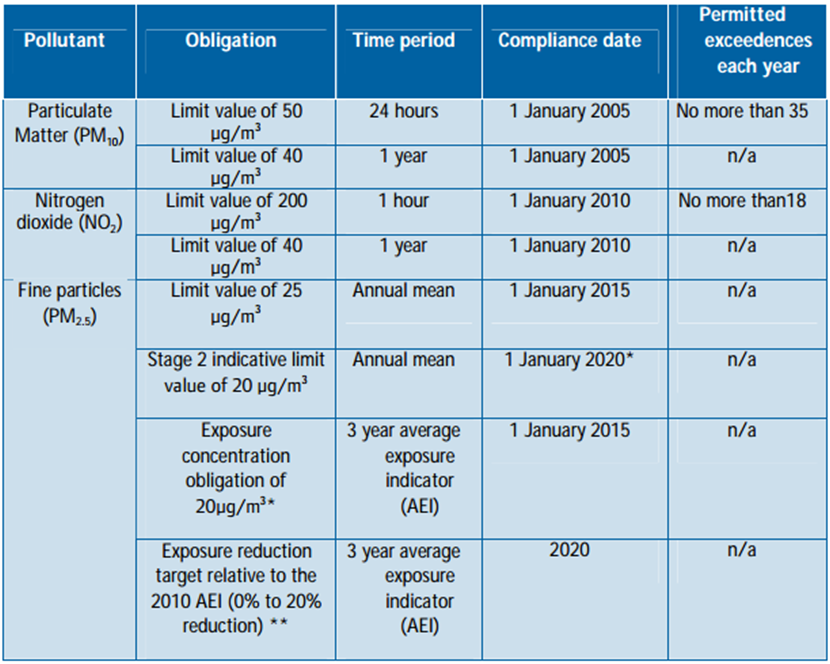
\includegraphics[scale=1]{eu_pm_limit_values}
\caption{EU Limit values for PM$_{2.5}$, PM$_{10}$ and NO$_{2}$}
\label{fig:eu_pm_limit_values}
\end{figure}

In addition, the 2010 Regulations state that sampling locations which are taken to be representative of exposure to humans must be sited to provide data on areas where the highest concentrations occur to which the population is likely to be exposed for a period which is significant in relation to the averaging period of any limit value.

Given the EU directives focus on PM10, PM2.5 and NO2, these are being targeted for reduction. As discussed in section \ref{subsec:trafficpollution} the main sources of these pollutants are traffic emissions

The overarching aim of this Strategy is to reduce air pollution in London so that the health of Londoners is improved. The most effective means to do this is to achieve the European Union (EU) air quality limit values as soon as possible.

\begin{figure}[H]
\centering
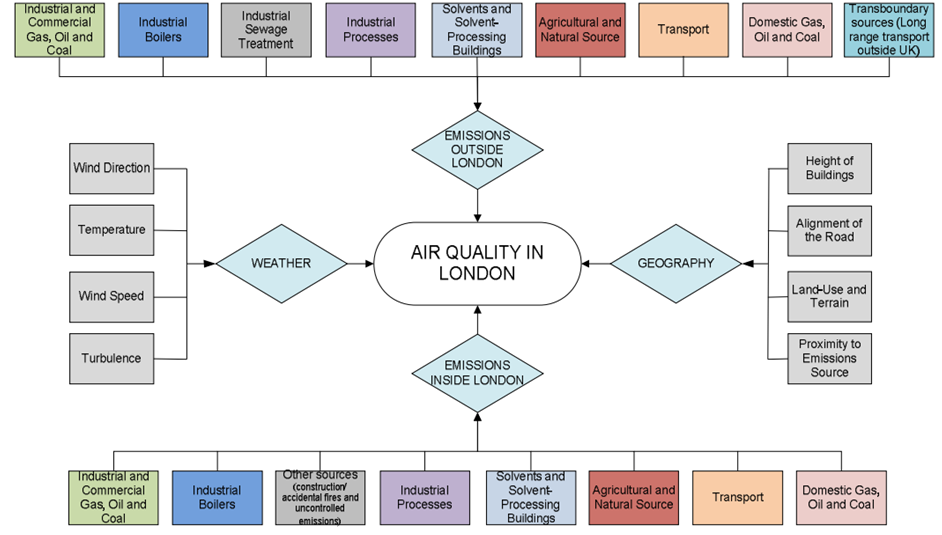
\includegraphics[scale=0.8]{what_influences_london_air}
\caption{What influences London's air quality from \cite{GreaterLondonAuthorityGLA2010}}
\label{fig:what_influences_london_air}
\end{figure}

\cite{GreaterLondonAuthorityGLA2010}
The challenge of cleaning London’s air is made more difficult because a significant amount of the pollution sources are not within London. Much is blown in from the surrounding regions including Europe, but some comes from much further away, from as far afield as the Sahara Desert. Around 40 per cent of NO2  pollution comes from emission sources outside London. Equally, data from central London indicates that about 40 per cent of PM10 originates from outside London. (Refer here to data collected by the London Air Quality Network, coordinated by King’s College London).

\begin{figure}[H]
\centering
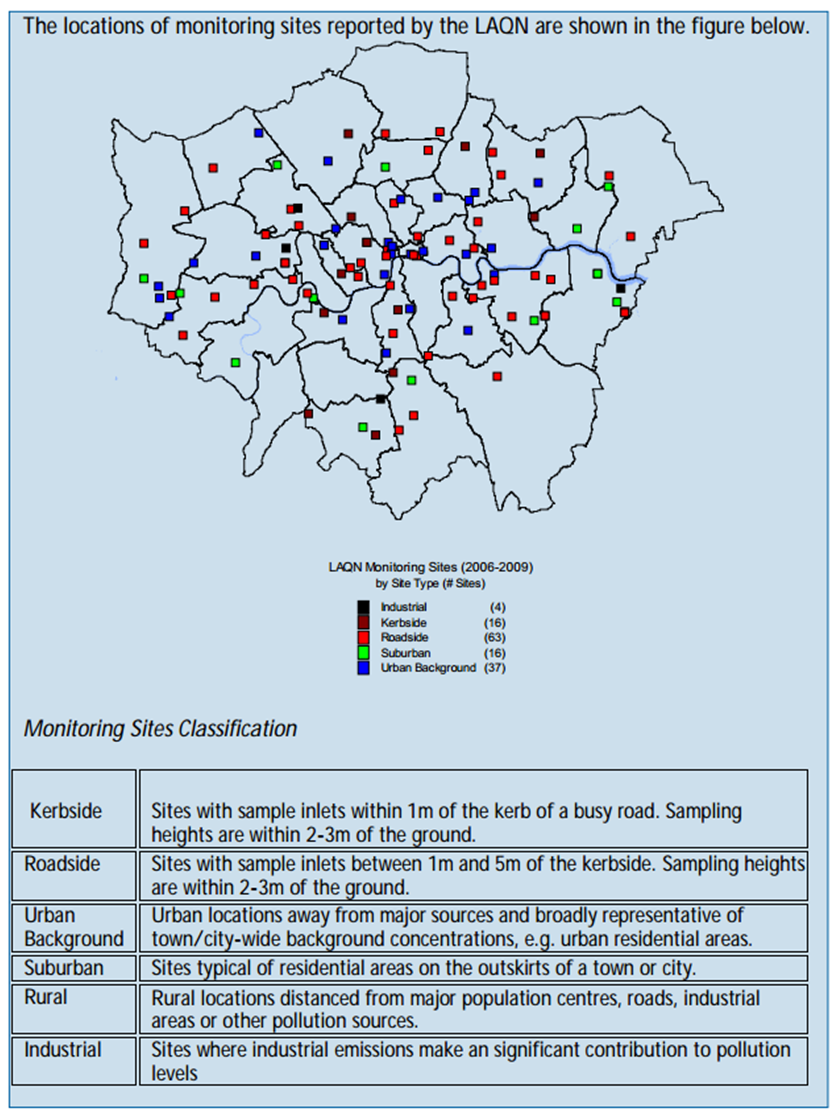
\includegraphics[scale=1]{laqn_monitoring_sites}
\caption{Not sure yet from \cite{GreaterLondonAuthorityGLA2010}}
\label{fig:laqn_monitoring_sites}
\end{figure}

\begin{figure}[H]
\centering
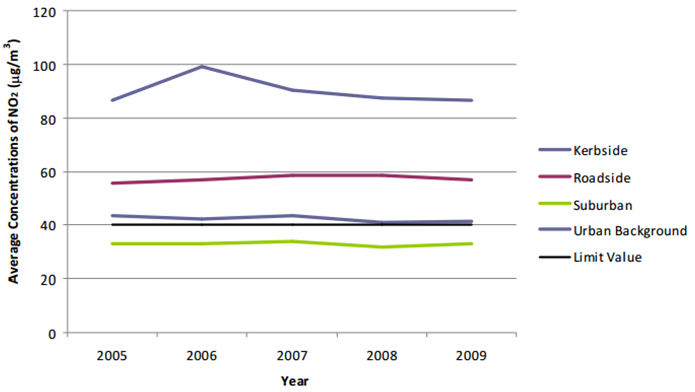
\includegraphics[scale=1]{london_yearly_no2}
\caption{Not sure yet from \cite{GreaterLondonAuthorityGLA2010}}
\label{fig:london_yearly_no2}
\end{figure}

\begin{figure}[H]
\centering
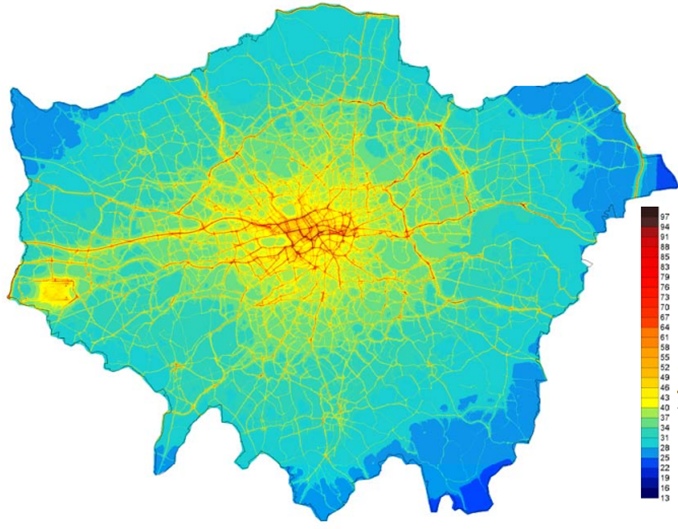
\includegraphics[scale=1]{modelled_london_no2_2008}
\caption{Modelled NO2 annual average concentrations (ug/m3) for the year 2008 from \cite{GreaterLondonAuthorityGLA2010}}
\label{fig:modelled_london_no2_2008}
\end{figure}

\begin{figure}[H]
\centering
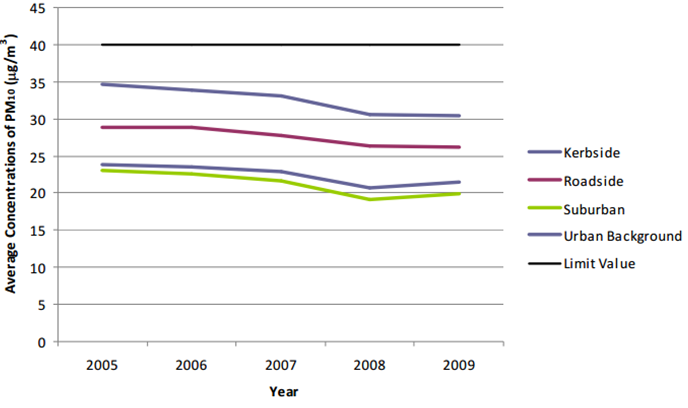
\includegraphics[scale=1]{london_yearly_pm10}
\caption{Not sure yet from \cite{GreaterLondonAuthorityGLA2010}}
\label{fig:london_yearly_pm10}
\end{figure}

\begin{figure}[H]
\centering
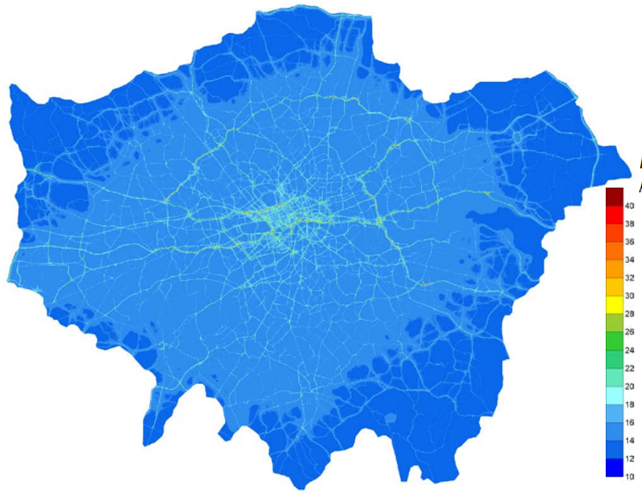
\includegraphics[scale=1]{modelled_london_pm10_2011}
\caption{Modelled PM10 annual mean concentrations (ug/m3) for the year 2011 from \cite{GreaterLondonAuthorityGLA2010}}
\label{fig:modelled_london_pm10_2011}
\end{figure}